\section{{\tt burn\_cell}}

\subsection{Getting Started}

The {\tt burn\_cell} codes are located in {\tt Microphysics/unit\_test/burn\_cell}. To run a simulation, ensure that both an input file and an initial conditions file have been created and are in the same directory as the executable. 

\subsection{Input File}

These files are typically named as {\tt inputs\_burn\_network} where {\tt network} is the network you wish to use for your testing.

The structure of this file is is fairly self-explanitory.
The run prefix defined should be unique to the tests that will be run as they will be used to identify all of the output files. Typically, the run prefix involves the name of the network being tested.
The {\tt atol} variables define absolute tolerances of the ordinary differential equations and the {\tt rtol} variables define the relative tolerances.
The second section of the input file collects the inputs that {\tt main.f90} asks for so that the user does not have to input all 5$+$ parameters that are required everytime the test is run.
Each input required is defined and initialized on the lines following {\tt \&cellparams}.
The use of the parameters is defined in Table~\ref{tab:init-structure}.

\begin{table}
	\centering
	\begin{tabular}{|l|l|}
		\hline
			\multicolumn{1}{|c|}{\textbf{Name in {\tt main.f90}}} &
			\multicolumn{1}{|c|}{\textbf{Definition}} \\
		\hline
		\rowcolor{tableShade}
		{\tt tmax} & Maximum Time (s) \\
		{\tt numsteps} & Number of time subdivisions \\
		\rowcolor{tableShade}
		{\tt density} & State Density ($\frac{g}{cm^3}$) \\
		{\tt temperature} & State Temperature (K) \\
		\rowcolor{tableShade}
		{\tt massfractions(i)} & Mass Fraction for element i \\
		\hline
	\end{tabular}
	\caption{The definition of parameters used in the {\tt burn\_cell} unit tests and specified in the second half of each inputs file.}
	\label{tab:init-structure}
\end{table}

\subsection{Running the Code}

To run the code, enter the {\tt burn\_cell} directory and run {\tt ./main.Linux.gfortran.exe} with the inputs file as an argument. 
For example: {\tt ./main.Linux.gfortran.exe inputs\_burn\_aprox13}

For however many events are run, defined as { \tt numsteps} in the inputs file, the code will output that many files into a new directory titled {\tt run\_prefix\_output} where {\tt run\_prefix} is the run prefix defined in the inputs file.
Each output file will be named using the run prefix defined in the inputs file and the corresponding timestep. 

Next, run {\tt burn\_cell.py} using Python3 and listing the defined run prefix as an argument.
For example: {\tt python3 burn\_cell.py react\_aprox13}. 
The burn\_cell code will gather information from all of the output files and compile them into three graphs explained below.

\subsection{Graphs Output by burn\_cell.py}

The file {\tt run-prefix\_logX.png} and {\tt run-prefix\_logX.eps} will display a graph of the chemical abundances as a function of the time, both on logarithmic scales, for all species involved in the simulation. 
An example of this graph is shown in Figure~\ref{fig:aprox13_logX}.

\begin{figure}
        \centering
	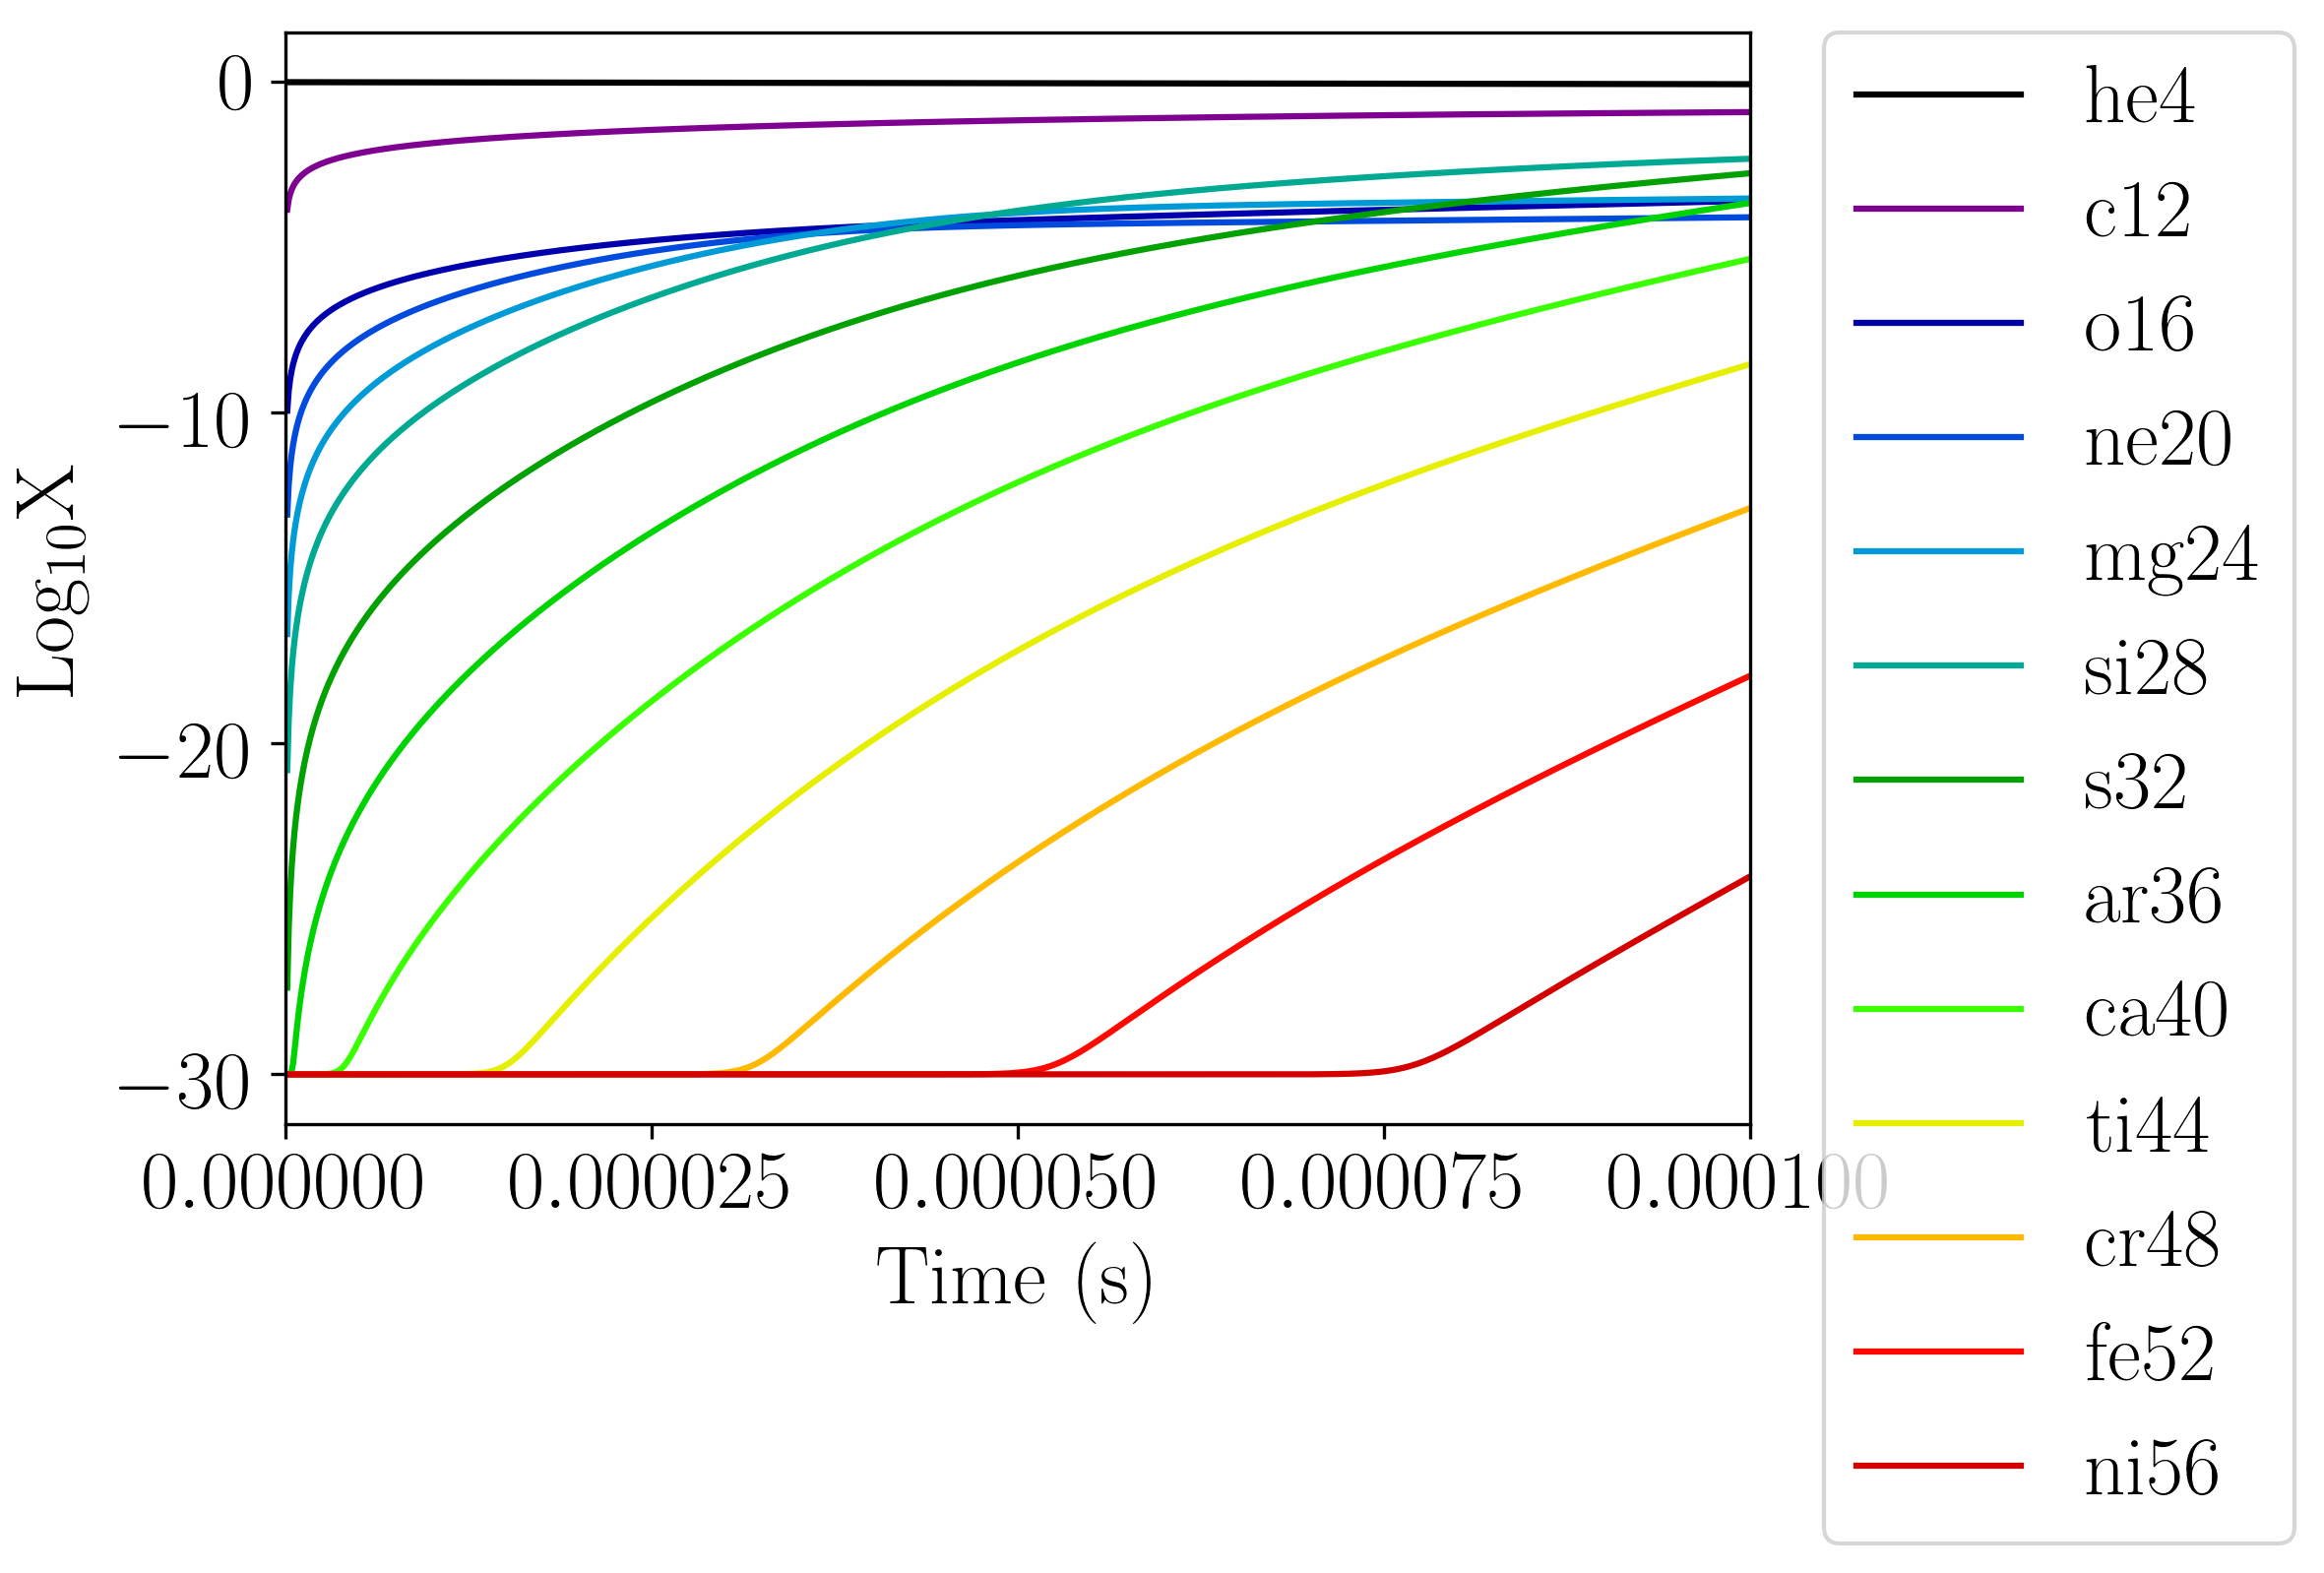
\includegraphics[width=4.5in]{react_aprox13_logX}
	\caption{An example of a plot output by the {\tt burn\_cell} unit test. This is the { \tt logX } output cooresponding to the network { \tt aprox13}.}
	\label{fig:aprox13_logX}
\end{figure}

The file {\tt run-prefix\_ydot.png} and {\tt run-prefix\_ydot.eps} will display the Moller fraction (mass fraction / atomic weight) as a function of time, both on logarithmic scales, for all species involved in the code. 

The file {\tt run-prefix\_T-edot.png} and {\tt run-prefix\_T-edot.eps} will display the Temperature and the Energy Generation Rate as a function of time. 
